\documentclass{beamer}
\beamertemplatenavigationsymbolsempty
\usepackage{amsmath, amssymb, hyperref, graphics}
\usepackage{graphicx}
\usepackage{tikz}
\usetikzlibrary{arrows}


\title{Graph Theory Lecture 7}

\begin{document}

\begin{frame}{Section 4: Graphs on Surfaces}
  \begin{block}{The Utilities Problem:}
  Connect three houses to three utilities without crossing the lines?
\begin{center}
  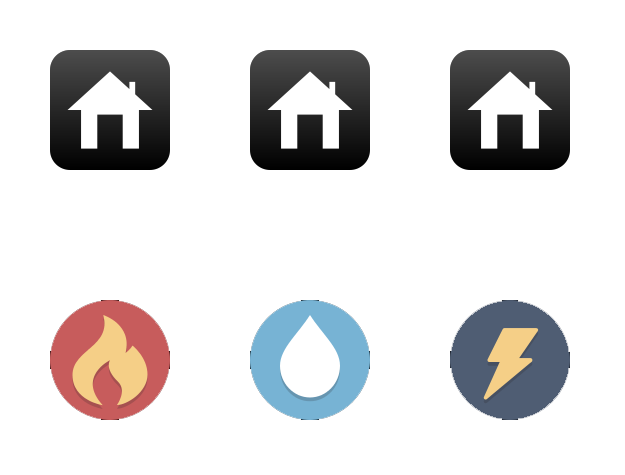
\includegraphics[width=.8\textwidth]{Pictures/utilities.png}
\end{center}
  \end{block}
 
 \end{frame} 


\begin{frame}{First, a definition}
  \begin{definition}A graph $G$ is \emph{planar} if it can be drawn in the plane so that no edges cross.
  \end{definition}

  \begin{block}{This ``definition'' is vague, fixing it requires analysis/topology}
    \begin{itemize}
    \item What do we mean ``draw'' an edge? 
      \begin{itemize}
        \item Injective continuous map $f:[0,1]\to\mathbb{R}^2$
        \end{itemize}
      \end{itemize}
    \end{block}
  \begin{block}{Not a course in topology; our intuition will be enough}
    \end{block}

  
  
\begin{block}{The Utilities question becomes:} Is the complete bipartite graph $K_{3,3}$ planar?
\end{block}
  


  \end{frame}


\begin{frame}{Isn't possible, but how to organize proof?}
  \begin{block}{Too many cases about how the edges could go...}
    Would be very lengthy, easy to miss a case.
  \end{block}

  \begin{block}{Instead, assume it was:}
    \begin{itemize}
      \item Any cycle $C_n\subset G$ would be drawn as a circle
      \item Any edge $e\in G, e\notin C_n$ would be inside or outside the circle
        \item Certain pairs of edges can't be on the same side...
\end{itemize}
    \end{block}

  \begin{block}{Mathematical culture:}
That a circle has two sides is surprisingly difficult topology.
    \begin{theorem}[Jordan curve theorem]
      A simple closed curve in the plane has an interior and an exterior
      \end{theorem}
    \begin{itemize}
    \item Simple: doesn't cross itself
    \item Closed: starts where it ends
    \end{itemize}




    \end{block}
  
\end{frame}

\begin{frame}{Theorem: $K_{3,3}$ isn't planar}
Let $A,B,C$ be blue vertices, $X,Y,Z$ be red.
  \begin{block}{Suppose $K_{3,3}$ were planar:}
    \begin{itemize}
    \item  Then the Hamiltonian cycle $AXBYCZA$ would be a circle
      \item The three edges $AY, BZ, CX$ still need to be drawn
\end{itemize}
    \end{block}
  \begin{block}{Case 1: $AY$ inside the cycle}
    \begin{itemize}
    \item But then we need to draw $BZ$ outside
    \item Two ways to do this, but either way can't draw $CX$
      \end{itemize}
  \end{block}
  \begin{block}{Case 2: $AY$ outside the cycle}
    \begin{itemize}
    \item Two ways to do this, but either way $BZ$ needs to be inside
    \item Now we can't draw $CX\quad\quad\square$
      \end{itemize}
\end{block}
  \begin{block}{The cases look awfully similar/redundant...}
    \end{block}

\end{frame}

\begin{frame}{From the plane to the sphere}
  \begin{block}{In the plane $\mathbb{R}^2$:}
    The outside and inside of a circle are different:
\begin{itemize}
\item    The inside is bounded, the outside isn't
  \item One way to connect inside, two ways to connect outside
\end{itemize}
\end{block}
  
  \begin{block}{But on the sphere $S^2$ things are nicer:}
    \begin{itemize}
    \item The ouside and inside of a circle look the same
    \item Only one way to connect outside      
    \end{itemize}
\end{block}
    \begin{block}{But we wanted to draw graphs on the plane, not the sphere}

      \end{block}
    \end{frame}

\begin{frame}{Stereographic projection: $S^2=\mathbb{R}^2\cup \{p\}$:}
  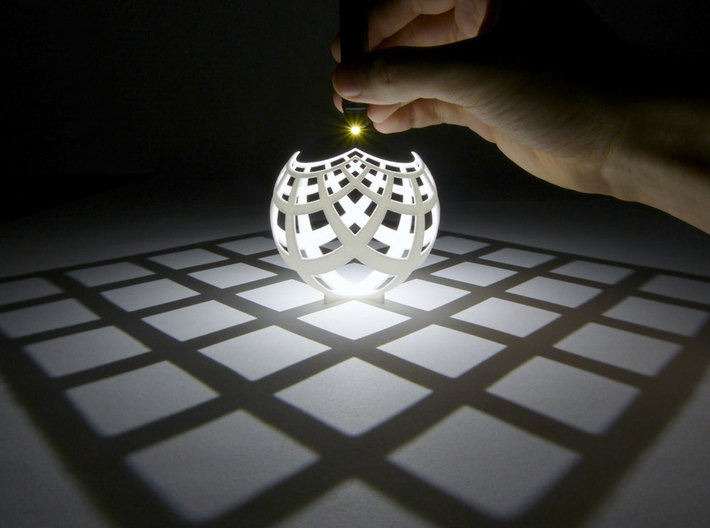
\includegraphics[width=.4\textwidth]{Pictures/stereographicSegerman.jpg}
  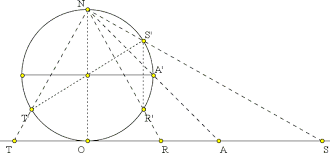
\includegraphics[width=.6\textwidth]{Pictures/stereographic2d.png}
\begin{corollary}
$G$ is planar if and only if $G$ can be drawn on the sphere.
  \end{corollary}
\begin{proof}
\begin{description}
    \item[If:] Draw $G$ on $S^2$; project from a point $p\in S^2\setminus G$
   \item[Only if:] Project from plane to sphere
     \end{description}
  \end{proof}
\begin{block}{Upshot: don't need to treat inside/outside as separate cases}
  \end{block}

\end{frame}

\begin{frame}{How far can we push and formalize this method?}

  \begin{itemize}
  \item $K_5$ isn't planar
  \item Petersen graph isn't planar
  \end{itemize}

  \begin{block}{Next time:}
    \begin{itemize}
    \item  This method is \emph{great} for Hamiltonian graphs
    \item What to do if you're far from Hamiltonian
\end{block}

\end{document}
